\begin{frame}{Conducting Research}
    Statistics permeates research from start to finish! 
    \begin{itemize}
        \item The first step in any experiment is to design it.
        \item We design an experiment by deciding
        \begin{enumerate}
            \item What we want to know.
            \item Our target population (who or what we want to know about).
            \item The statistical methods we will use to analyze our data (this helps us decide what kind of data to collect).
        \end{enumerate}
    \end{itemize}
\end{frame}

\begin{frame}{Choosing How to Collect Data}
    A clear, specific research question can go a long way in helping to identify what subjects/cases are important and which variables we should measure. 
    
    \vspace{12pt}
    But we also need to consider \textit{how} these variables are measured.
\end{frame}

\begin{frame}{Research Questions}
    \begin{itemize}
        \item Research questions ask a question about some target \textbf{population}, which can be made up of anything we are interested in - people, dogs, bicycles, you name it.
        \item Typically we don't have access to every single person/dog/case in a population, so instead we look at a subset of the population. 
        \item This subset is called a \textbf{sample}. It is often a small fraction of the total population.  
    \end{itemize}
\end{frame}

\begin{frame}{Research Questions}
    Let's think about some possible research questions:
    \begin{enumerate}
        \item What is the average mercury content in swordfish in the Atlantic Ocean?
        \item Over the last 5 years, what is the average time to complete a degree for UCR undergrads?
        \item Does a new drug reduce the number of deaths in patients with severe heart disease?
    \end{enumerate}
    
    \vspace{12pt}
    What makes these research questions clear and specific? 
\end{frame}

\begin{frame}{Populations and Samples}
    What is the average mercury content in swordfish in the Atlantic Ocean?
    
    \begin{itemize}
        \item What is the target population in this research questions?
        \item What would represent an individual case?
    \end{itemize}
\end{frame}

\begin{frame}{Populations and Samples}
    What is the average mercury content in swordfish in the Atlantic Ocean?
    
    \begin{itemize}
        \item What is the target population in this research questions?
        \begin{itemize}
            \item All swordfish in the Atlantic Ocean.
        \end{itemize}
        \item What would represent an individual case?
        \begin{itemize}
            \item Each individual swordfish in the Atlantic Ocean.
        \end{itemize}
    \end{itemize}
\end{frame}

\begin{frame}{Populations and Samples}
    Discuss with a neighbor and jot down your thoughts on our other two research question examples. What is the target population in each research question? What represents an individual case?
    
    \vspace{12pt}
    1. Over the last 5 years, what is the average time to complete a degree for UCR undergrads?
    
    2. Does a new drug reduce the number of deaths in patients with severe heart disease?
    
\end{frame}

\begin{frame}{Populations and Samples}
    1. Over the last 5 years, what is the average time to complete a degree for UCR undergrads?
    \begin{itemize}
        \item Population: all UCR undergrads
        \item Individual case: each UCR undergrad
    \end{itemize}
\end{frame}

\begin{frame}{Populations and Samples}
    2. Does a new drug reduce the number of deaths in patients with severe heart disease?
    \begin{itemize}
        \item Population: all patients with severe heart disease
        \item Individual case: each patient with severe heart disease
    \end{itemize}
\end{frame}

\begin{frame}{Anecdotal Evidence}
    Consider the following:
    \begin{enumerate}
        \item I ate Atlantic swordfish and got mercury poisoning, so the mercury levels must really high. 
        \item I know of two UCR undergrads who took 8 years to graduate, so it must take an unusually long time to graduate from UCR.
        \item My dog took a new heart disease drug and hasn't had a heart attack, so it must work.
    \end{enumerate}
\end{frame}

\begin{frame}{Anecdotal Evidence}   
    \vspace{12pt}
    Each claim on the previous slide is based on data! But...
    \begin{enumerate}
        \item The sample sizes are very small!
        \item Even if we manage to verify these claims (e.g., the mercury poisoning was actually caused by swordfish), we have no way of knowing if they represent the population well or are extreme cases.
        \item We often remember only the extreme cases because they are striking (or possibly due to expectation bias).
    \end{enumerate}
    
    \vspace{12pt}
    Can you think of a time when you heard someone to use \textbf{anecdotal evidence} to demonstrate a point?
\end{frame}

\begin{frame}{Sampling from a Population}
    One we've established our target population and what constitutes an individual case, it's time to think about collecting a sample. 
    
    \vspace{12pt}
    For our question about UCR time-to-graduation, recall that
    \begin{itemize}
        \item our \textit{population} is all UCR undergrads
        \item and our \textit{sample} is made up of whatever graduated students we selected for review.
    \end{itemize}
\end{frame}
 
\begin{frame}{Sampling from a Population}    
    \vspace{12pt}
    What if we took a sample of everyone in an upper division physics course? Are these students likely to be representative of UCR students \textit{on average}?
\end{frame}
 
\begin{frame}{Sampling from a Population}     
    \vspace{12pt}
    If we select samples this way, we are likely to get a \textbf{biased} sample. In this case, we would \textit{bias} the sample toward however long it takes physics students to graduate. 
\end{frame}

\begin{frame}{Sampling from a Population}
    In order to get a sample that represents UCR students overall, we want to \textit{randomly} sample from our population of all graduated UCR undergrads.
    
    \vspace{12pt}
    Think of a random sample as a raffle. Each graduated UCR student from the past 5 years get a raffle ticket, and 100 of them are selected randomly. We then ask these 100 students how long they took to graduate. 
\end{frame}

\begin{frame}{The Simple Random Sample}
    The most straightforward way to collect a random sample is the \textbf{simple random sample}. This is essentially equivalent to the raffle example:
    \begin{itemize}
        \item Each case in the population has an equal probability of being included in the sample.
        \item There is no connection between cases in the sample.
    \end{itemize}  
\end{frame}

\begin{frame}{Sources of Bias}
    \textbf{Bias} can occur in simple random samples due to individuals not responding. 
    
    \vspace{12pt}
    If students who took 6 or more years to graduate also happen to be less likely to respond, we may end up with data to suggest that our average time-to-graduation is quicker than it actually is. 
\end{frame}

\begin{frame}{Sources of Bias}   
    \vspace{12pt}
    Usually bias occurs in a sample when we do something out of convenience instead of going through all of the steps to get a truly random sample. 
    
    \vspace{12pt}
    A \textbf{convenience sample} is where individuals are sampled because it's easy. E.g., you sample everyone in this class instead of trying to randomly sample from all UCR students. 
\end{frame}

\begin{frame}{Bias in the Wild: Amazon Reviews}
    \begin{columns}[T] % align columns
    \begin{column}{.48\textwidth}
        \vspace{2cm}
        
        Suppose you're looking for a new outfit for your pet lizard. You find what appears to be the perfect outfit on Amazon, but the reviews are pretty mixed.
    \end{column}%
    \hfill%
    \begin{column}{.48\textwidth}
    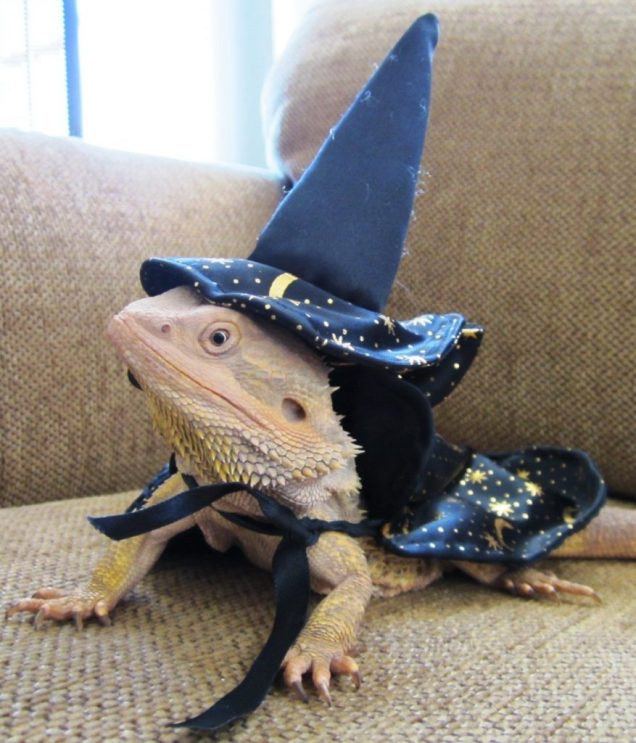
\includegraphics[scale=0.25]{images/lizard.jpg}
    \end{column}%
    \end{columns}
\end{frame}

\begin{frame}{Bias in the Wild: Amazon Reviews}
        \begin{columns}[T] % align columns
    \begin{column}{.48\textwidth}
        \vspace{2cm}
    
        Do you think the reviews give an accurate representation of how buyers feel about this item? When do you think people are more likely to leave reviews?
    \end{column}%
    \hfill%
    \begin{column}{.48\textwidth}
    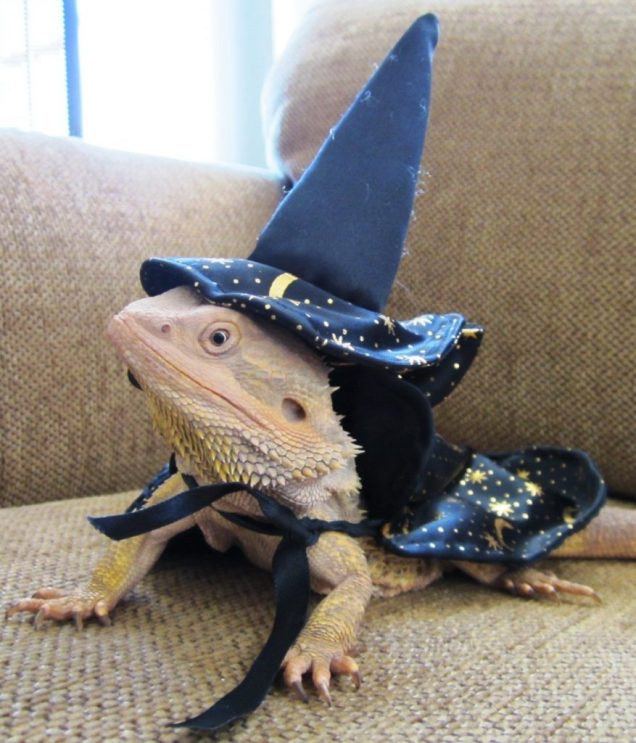
\includegraphics[scale=0.25]{images/lizard.jpg}
    \end{column}%
    \end{columns}
\end{frame}

\begin{frame}{Observational Studies}
    Data where no treatment is explicitly applied (or withheld) is \textbf{observational data}. 
    \begin{itemize}
        \item These kinds of studies are \textit{non-experimental}.
        \item It is difficult to make causal claims based on observational data.
        \item Instead, we can use observational studies to 
        \begin{itemize}
            \item form hypotheses for future experiments.
            \item demonstrate associations (that may or may not be causal).
        \end{itemize}
    \end{itemize}
\end{frame}

\begin{frame}{Examples of Observational Studies}
    \begin{itemize}
        \item Relationship between smoking and lung health.
        \begin{itemize}
            \item Here, smoking is the "treatment".
            \item Ethical constraints prevent us from randomly assigning people to smoking or nonsmoking.
        \end{itemize}
        \item Relationship between gender and number of pets.
        \begin{itemize}
            \item Here, gender is the "treatment".
            \item We can't impose a gender on someone, so we are unable to randomly assign gender.
        \end{itemize}
    \end{itemize}
\end{frame}

\begin{frame}{Observational Studies}
    Can you think of something you might be interested in studying where "treatment" can't be explicitly applied? 
    
    \vspace{18pt}
    How do you think we deal with some of the ethical constraints like those in the smoking study? 
\end{frame}

\begin{frame}{Why No Causal Claims?}
    Consider an observational study that tracked sunscreen use versus skin cancer. The study found that the more sunscreen someone used, the more likely they were to develop skin cancer. 
    
    \begin{itemize}
        \item Does sunscreen use cause skin cancer?
        \item What information could we be missing?
    \end{itemize}
\end{frame}

\begin{frame}{Sunscreen and Skin Cancer}
    \begin{itemize}
        \item This missing information consists of variables that we didn't measure.
        \textbf{Confounding variables} are variables that are correlated with (have a relationship with) both the explanatory and response variables.
        \item Confounding variables can help explain why unexpected relationships occur.
        \item It is almost impossible to guarantee that we've measured (or even thought of) all confounding variables.
        \item Note: just because a relationship makes sense, doesn't mean it is causal or that there are no confounding variables!
    \end{itemize}
\end{frame}

\begin{frame}{Types of Observational Studies}
    We can ask two types of observational questions. 
    \begin{itemize}
        \item A \textbf{prospective study} collects data as the events unfold.
        \item A \textbf{retrospective study} collects data on events that have already taken place. 
    \end{itemize}
    
    Some datasets may include variables taken both prospectively and retrospectively. 
\end{frame}

\begin{frame}{Sampling Methods}
    \textbf{Simple random sampling} is the "raffle method" we talked about earlier. Each case has an equal probability of being selected from the population.
    
    \vspace{18pt}
    \textbf{Stratified sampling} uses a "divide-and-conquer" approach. 
    \begin{itemize}
        \item The population is divided into groups called \textbf{strata}, chosen so that similar cases are grouped together.
        \begin{itemize}
            \item We could group based on variables like year in college, gender, team, etc.
            \item We typically choose these grouping based on some variable that we think relates to our outcome. 
        \end{itemize}
        \item We then randomly sample a fixed number of cases from each strata. 
    \end{itemize}
\end{frame}

\begin{frame}{Sampling Methods}
    \textbf{Cluster sampling} involves breaking the population into many groups, called \textbf{clusters}. 
    \begin{itemize}
        \item We then randomly select some of the clusters and sample all of the cases in each of the selected clusters.
    \end{itemize}
    
    \vspace{18pt}
    \textbf{Multistage sampling} is similar to cluster sampling, but instead of keeping all cases in each cluster, we randomly sample from each selected cluster (this is the "multistage" part). 
\end{frame} 

\begin{frame}{Sampling Methods}
    Cluster and multistage sampling may be cheaper and easier to collect.
    \begin{itemize}
        \item If we wanted to sample individuals from 30 remote villages, it would be cheaper to cluster by village and only travel to 10 of them. 
    \end{itemize}
    We may also use these approaches when within-cluster variability is high but the clusters are similar \textit{on average}. 
    \begin{itemize}
        \item For example, 5 economically diverse neighborhoods with similar average wages in each neighborhood. 
    \end{itemize}
    
    \vspace{18pt}
    The analyses discussed in this class will all pertain to simple random sampling. However, most of these analyses can be extended to work with a variety of sampling methods. 
\end{frame}